Load-balancing problems can be formulated in many ways. This is
especially true for the case addressed in this paper where the
load-balancer should distribute the load to adaptive entities, that
play a role by themselves in adjusting to the current situation. This
section discusses the characteristics of the considered infrastructure
and clearly formulate the problem under analysis.

\begin{figure}[t]
  \centering 
  \usetikzlibrary{arrows}
\usetikzlibrary{automata}
\usetikzlibrary{positioning}
\usetikzlibrary{backgrounds}
\usetikzlibrary{fit}

\tikzset{
    state/.style={
           rectangle,
           rounded corners,
           draw=black, very thick,
           minimum height=0.6cm,
           minimum width=1cm,
           inner sep=3pt,
           text centered,
           node distance=0.9cm,
           },
    process/.style={
           rectangle,
           rounded corners,
           draw=black, very thick,
           minimum height=0.6cm,
           minimum width=1cm,
           inner sep=3pt,
           text centered,
           %node distance=1cm,
           },
    newprocess/.style={
           rectangle,
           rounded corners,
           draw=black, very thick,
           fill=lightgray,
           minimum height=0.6cm,
           minimum width=1cm,
           inner sep=3pt,
           text centered,
           %node distance=1cm,
           },
    processplaceholder/.style={
           minimum height=0.6cm,
           minimum width=1cm,
           %inner sep=3pt,
           text centered,
           %node distance=1cm,
           },
    closerstate/.style={
           rectangle,
           rounded corners,
           draw=black, very thick,
           minimum height=0.5cm,
           minimum width=5.32cm,
           inner sep=3pt,
           text centered,
           node distance=1cm,
           },
    abovish/.style={
           rectangle,
           rounded corners,
           draw=none,
           minimum width=1cm,
           text centered,
           node distance=1cm,
           },
    supercloserstate/.style={
           rectangle,
           draw=none,
           minimum height=0.2cm,
           minimum width=6.9cm,
           node distance=1cm,
           },
}

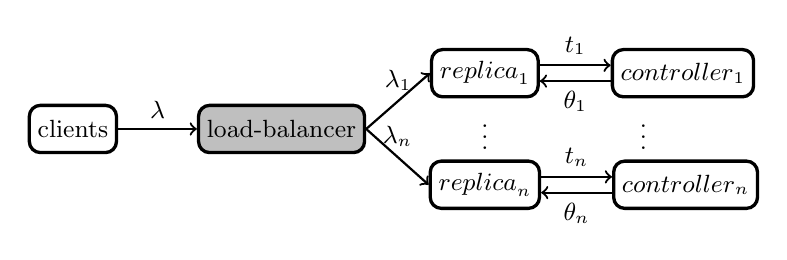
\begin{tikzpicture}[font=\small]
  \tikzstyle{surround} = [fill=black!20,very thick,draw=black,rounded
  corners, inner sep=5pt,] \tikzstyle{surroundblue} =
  [fill=blue!20,very thick,draw=black,rounded corners, inner sep=5pt,]
  \tikzstyle{surroundyellow} = [fill=yellow!20,very
  thick,draw=black,rounded corners, inner sep=5pt,]
  \tikzstyle{external} = [fill=none,very thick,draw=black,rounded
  corners, inner sep=15pt,]

% clients
\node[process] (clients){clients};

% load-balancer
\node[newprocess, right=1cm of clients] (lb){load-balancer};

% servers
\node[processplaceholder, right=1cm of lb] (replicaI) {$\vdots$};
\node[process, above=0cm of replicaI] (replica1) {$\text{replica}_1$};
\node[process, below=0cm of replicaI] (replicaN) {$\text{replica}_n$};

% controllers
\node[processplaceholder, right=1cm of replicaI] (controllerI) {$\vdots$};
\node[process, right=0.9cm of replica1] (controller1) {$\text{controller}_1$};
\node[process, right=0.9cm of replicaN] (controllerN) {$\text{controller}_n$};

% clients to lb
\draw[thick,->] (clients.east) -- (lb.west) node[midway, above] {$\lambda$};

% lb to replicas
\draw[thick,->] (lb.east) -- (replica1.west) node[midway, above] {$\lambda_1$};
\draw[thick,->] (lb.east) -- (replicaN.west) node[midway, above] {$\lambda_n$};

% replica to controllers
\draw[thick,->] ([yshift=+1mm]replica1.east) -- ([yshift=+1mm]controller1.west) node[midway, above] {$t_1$};
\draw[thick,<-] ([yshift=-1mm]replica1.east) -- ([yshift=-1mm]controller1.west) node[midway, below] {$\theta_1$};
\draw[thick,->] ([yshift=+1mm]replicaN.east) -- ([yshift=+1mm]controllerN.west) node[midway, above] {$t_n$};
\draw[thick,<-] ([yshift=-1mm]replicaN.east) -- ([yshift=-1mm]controllerN.west) node[midway, below] {$\theta_n$};

\end{tikzpicture}
 
  \caption{Architecture of a brownout-compliant cloud application
    featuring multiple replicas.}
  \label{fig:architecture}
\end{figure}

Figure~\ref{fig:architecture} illustrates the software architecture
that is deployed to execute a brownout-compliant application composed
by multiple replicas. Despite the modifications needed to make it
brownout-compliant, the architecture is widely accepted as the
reference one for cloud applications~\citep{Barroso09}.

In a generic load-balancing infrastructure, clients generate traffic
to the cloud application at an unpredictable but measurable rate
$\lambda$. The traffic is directed to a load-balancer that sorts it,
sending requests to the different $n$ replicas. Each replica $i$
receives a fraction $\lambda_i$ of the incoming traffic and implements
the application logic. Clearly, since the load balancer is redirecting
the entire pool of received requests, $\sum_i \lambda_i = \lambda$.
It is also possible to formulate the problems using replica weights.
In this case, each replica receives requests at a rate $\lambda_i =
w_i \cdot \lambda$, such that $\sum_{i} w_i = 1$. In this case, the
load balancer simply computes the \textbf{replica weights} $w_i$
according to its load-balancing policy.

Special to our case is the presence of a controller within each
replica~\cite{cloudish-tr}. This controller takes care of adjusting
the percentage of requests served with the optional components enabled
based on the measured response time of the requests served by the
replica. The controller for replica $i$ receives a vector of response
times $t_i$ (the average value can be used, as well as the maximum one
or the 99th percentile, depending on what the requirements on the
control systems are) and produces the percentage $\theta_i$ of
requests that should be served with optional components in the next
time interval.

In fact, a replica $i$ responds to requests either partially, where
only mandatory content is included in the reply, or fully, where both
mandatory and optional content is included. The service rate for a
partial response is $\mu_i$ while a full response is generated with a
rate $M_i$. Obviously, partial replies are faster to compute than full
ones, since the optional content does not need to be prepared, hence,
$\mu_i \geq M_i$. Assuming the replica is not saturated, it serves
requests fully at a rate $\lambda_i \cdot \theta_i$ and partially at a
rate $\lambda_i \cdot (1-\theta_i)$. An existing load-balancer based
on response times analysis would hardly work with brownout-compliant
applications, due to their self-adaptivity and the selection of the
value $\theta_i$.

Many alternatives can be envisioned on how to extend existing load
balancers to deal with brownout-compliant applications.

In the first case, the load-balancer does not know anything about the
current state of the system but can inspect the requests and the
responses and see how many of them have been executed with the
optional components turned on. This would give it an estimation of the
probability of executing optional code $\theta_i$ per replica but not
the certainty of its current value, due to the probabilistic setup.

In the second case, the load-balancer does not know anything about the
state of the system and cannot inspect the requests because this would
be too heavy on the architecture, therefore it can try to estimate the
probability of executing optional code based on the time needed to
compute the response --- clearly, a request with optional code enabled
would take longer than one without it. The estimate of $\theta_i$ in
this case would be less accurate than in the previous scenario.

In the third scenario, the load-balancer receives information about
$\theta_i$ from the replicas. This solution is lighter than the others
on the load balancer side but requires additional communication. The
overhead, however, is very limited, since only one value should be
reported per replica. For the purposes of this paper, we assume that
to aid load-balancing decisions, each replica piggy-backs the current
value of $\theta_i$ through the reply, so that this value can be
observed by the load-balancer, limiting the overhead. The parameters
$\theta_i$ are computed by controllers based on a target average or
maximum response time $\bar{\tau}$. Each replica $i$ periodically
reports the average observed vector of response-times $t_i$ to its
controller. In exchange, the controller adjusts $\theta_i$ to maintain
the desired response-time close to its target value. The load-balancer
does not have any knowledge on \emph{how} each replica controller
adjusts the percentage $\theta$, it can only know its reported value.

Within this architecture, we want to solve the problem of designing a
{\bf load-balancer policy}. Knowing the values of $t_i$ and $\theta_i$
for each replica $i \in [1, n]$ and the current (assumed constant)
arrival rate $\lambda$, a load-balancer should compute the values of
the weights $w_i$ such that
\begin{equation}
\sum_{i} \lambda w_i \theta_i = \lambda \sum_i w_i \theta_i
\label{eq:objective}
\end{equation}
is maximized. In other words, the load-balancer should maximize the
amount of requests served with the optional part enabled. In practice,
this would also maximize the application owner's revenue.
